\documentclass[11pt]{article}
\usepackage[a4paper,left=1in,right=1in,top=1in,bottom=1in]{geometry}

\usepackage[english]{babel}
\usepackage[T1]{fontenc}
\usepackage[utf8]{inputenc}
\usepackage{seqsplit}

\renewcommand{\familydefault}{\sfdefault}
\usepackage{setspace}  \singlespacing
\usepackage{graphicx}
\usepackage[absolute]{textpos}
\usepackage{xcolor}
\usepackage{fontawesome5}
\usepackage{multirow}
\usepackage{hyperref}
\usepackage{tcolorbox}
\hypersetup{
    colorlinks,
    linkcolor={red!50!black},
    citecolor={blue!50!black},
    urlcolor={blue}
}

\definecolor{mgray}{gray}{0.85}
\definecolor{mpurple}{HTML}{68236D}
% Additional packages for the content
\usepackage{float}
\usepackage{subfig,wrapfig}
\usepackage{amsmath,amsfonts,amsthm,amssymb}
\usepackage{fancyhdr,fancybox,color}
\usepackage{enumerate}
\usepackage[amssymb]{SIunits}
\definecolor{MyBlue}{rgb}{0,0.3,0.6}
\usepackage[all]{hypcap}
\usepackage{csquotes}
\usepackage[url=false,
backend=bibtex,
style=authoryear-comp,
doi=true,
isbn=true,
backref=false,
dashed=false,
maxcitenames=2,
maxbibnames=99,
natbib=true]{biblatex}
\DeclareNameAlias{author}{family-given}
\renewbibmacro{in:}{}
\addbibresource{../_logosAndRef/references.bib}
\nonfrenchspacing

% Configurable separation between header and body
\newlength{\headertobodysep}
\setlength{\headertobodysep}{1cm}

% Header with logos and contact information
\begin{document}
\thispagestyle{empty}

% Lean header with aligned elements
\textblockorigin{0pt}{0pt}

% Durham logo on the left
\begin{textblock*}{5cm}(0.5cm,1cm)
    
\includegraphics[height=2cm]{../_logosAndRef/Durham-University.pdf}
\end{textblock*}

% Contact information in the center - vertically centered with logos
\begin{textblock*}{9cm}(6cm,1.5cm)
    \centering
    {\large \textbf{Viscoelastic Singularities | CoMPhy Lab}}\\[0.2em]
    Department of Physics, Durham University\\[0.3em]
    \href{https://comphy-lab.org}{comphy-lab.org}
\end{textblock*}

% CoMPhy logo aligned with right margin
\begin{textblock*}{5cm}(15.5cm,1cm) % exactly 1 cm away from the right edge
    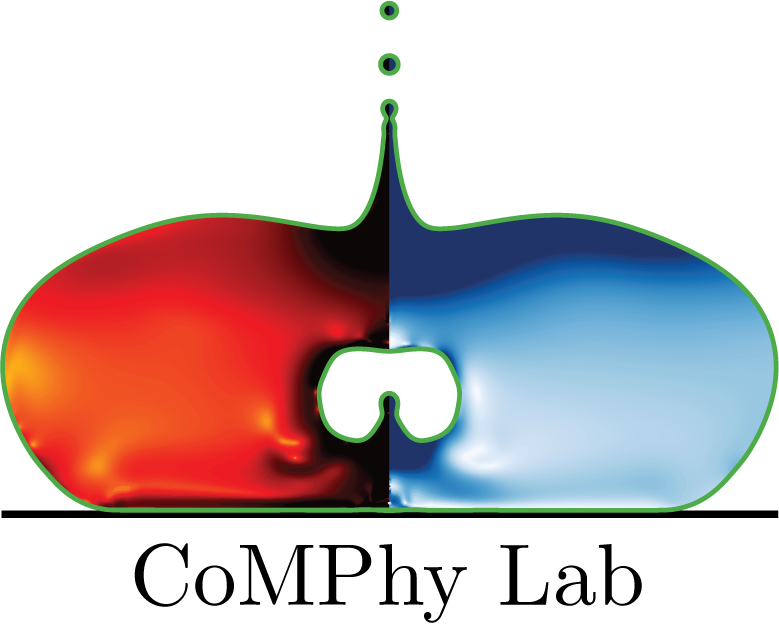
\includegraphics[height=2cm]{../_logosAndRef/CoMPhy-Lab.png}
\end{textblock*}

% Reset to normal text flow after header
\vspace*{\headertobodysep}

\begin{center}
    \begin{LARGE}
     Singularities in soft matter: how rheology picks the pinch-off exponent
    \end{LARGE}
\end{center}

\noindent Pull a thread of shampoo apart between two fingers and watch what the last millisecond does. A column of water would thin smoothly into a cusp and separate, obeying the self-similar pinch-off law Eggers wrote down thirty years ago~\citep{eggers1993universalPinchOff}. Shampoo does almost nothing of the sort. The thread stalls, elastic stress builds, a uniform cylindrical filament forms and thins exponentially in time, beads appear along it, and only then --- sometimes --- does it break. At no point in continuum mechanics does a fluid's rheology speak more unambiguously than at the instant of breakup. The Newtonian answer is a theorem~\citep{eggers2015singularities}. The viscoelastic answer is an open zoo. Different constitutive models --- Oldroyd-B, Giesekus, Johnson--Segalman, Rolie--Poly, soft-glassy rheology --- either regularise the singularity, re-select its exponents, or forestall it entirely through an extensional necking instability that breaks the filament before a singular point can form~\citep{fielding2011necking}. This project charts, for the first time end-to-end with direct numerical simulation carried all the way to breakup, which of those three fates each model selects, and where in $(Wi, De, Ec)$ the boundaries lie.

\begin{tcolorbox}[colback=mgray,colframe=mpurple,title=TL;DR]
Newtonian filament pinch-off has a textbook self-similar answer~\citep{eggers1993universalPinchOff,eggers2015singularities}; viscoelastic pinch-off does not. Which of three fates a thread selects --- a regularised (non-singular) Oldroyd-B exponential thinning~\citep{entovHinch1997}, a re-selected singular exponent at finite polymer extensibility (Giesekus, FENE-P), or collapse through an extensional necking instability that kills the filament before the singularity forms~\citep{fielding2011necking,hoyleFielding2016necking} --- is set by the constitutive law, the finite-extensibility ingredient, and shear-banding~\citep{wilsonFielding2006}. Governing groups are the Ohnesorge number $Oh = \mu/\sqrt{\rho\gamma R_0}$, the Weissenberg number $Wi = \lambda\dot\varepsilon$, the Deborah number $De = \lambda/\tau_{\mathrm{cap}}$ with $\tau_{\mathrm{cap}} = \sqrt{\rho R_0^3/\gamma}$, and the elasto-capillary number $Ec = G R_0/\gamma$. You will benchmark the Newtonian Eggers solution and the Entov--Hinch exponential regime in Basilisk C, implement a ladder of constitutive models (Oldroyd-B~\citep{entovHinch1997}, Giesekus/FENE-P~\citep{bhat2010beads}, Johnson--Segalman~\citep{wilsonFielding2006}, Rolie--Poly~\citep{likhtmanGraham2003roliepoly}, soft-glassy rheology~\citep{sollich1997sgr}) in the log-conformation formulation~\citep{fattalKupferman2004logconf} to keep polymer stress stable at large $Wi$, sweep the $(Wi, De, Ec)$ plane, and benchmark against the classical CaBER methodology~\citep{mckinleyTripathi2000caber}. Outputs: a regime map of viscoelastic singularity classes, a peer-reviewed paper co-supervised with Prof.\ Suzanne Fielding's group, and an open-source CoMPhy-Lab workflow.
\end{tcolorbox}

\section*{Description}

Every fluid knows how to break, and the instant of failure is the only place in continuum mechanics where rheology speaks for itself. For a Newtonian thread the answer is textbook: a self-similar pinch-off with universal exponents, derived from the $(\eta, \gamma, \rho)$ balance in a narrowing neck and verified to within a few percent in experiment~\citep{eggers1993universalPinchOff,eggers2015singularities}. The viscoelastic case is an open zoo. Some polymer threads refuse to break at all over any experimentally accessible timescale. Others bead up into a chain of droplets connected by ever-thinner cylindrical ligaments~\citep{bhat2010beads}. Others collapse through an extensional necking instability well before the singularity forms, producing a heterogeneous filament that breaks at a chosen weakest point rather than at a generic self-similar cusp~\citep{fielding2011necking,hoyleFielding2016necking}. Which of those fates a fluid selects depends entirely on its constitutive law, and pinch-off is the sharpest experimentally accessible test of that law there is.

Three dimensionless groups govern the problem once the geometry and bulk viscosity are fixed. The Ohnesorge number $Oh = \mu/\sqrt{\rho\gamma R_0}$ sets viscous forces against the inertial--capillary scale and distinguishes inertial from viscous Newtonian pinch-off. The Weissenberg number $Wi = \lambda\dot\varepsilon$ compares polymer relaxation against the instantaneous deformation rate in the neck; it is not externally imposed but rises as the neck thins, and any constitutive model must be integrated forward until $Wi$ passes through whichever finite-extensibility ceiling it imposes. The Deborah number $De = \lambda/\tau_{\mathrm{cap}}$ with capillary time $\tau_{\mathrm{cap}} = \sqrt{\rho R_0^3/\gamma}$ ranks relaxation against the thread's natural capillary-wave timescale. The elasto-capillary number $Ec = G R_0/\gamma$ weighs the polymer modulus $G$ against Laplace pressure; in the exponentially thinning regime the thread radius follows $R(t)/R_0 \sim \exp(-t/3\lambda)$, and $Ec$ sets the crossover at which that elastic regime begins~\citep{entovHinch1997}. The fourth group --- the retardation or finite-extensibility parameter of the chosen constitutive law --- is the one that actually selects the breakup scenario.

The constitutive ladder encodes the scientific question. Oldroyd-B isolates linear elasticity and predicts Entov--Hinch exponential thinning, which never reaches a singular point in finite time~\citep{entovHinch1997}: the singularity is \emph{regularised}. Giesekus and FENE-P reinstate a finite polymer-extension ceiling; once the stretch saturates, the thread can pinch off again, but with a \emph{re-selected} exponent that depends on the saturation law; this is the regime in which beads-on-a-string chains form~\citep{bhat2010beads}. Johnson--Segalman introduces a non-monotonic flow curve and admits shear-banded solutions; its relevance to filament breakup is not that shear bands form in extension (they do not), but that the same non-monotonicity that supports shear banding in simple shear drives an extensional necking instability whose signatures Prof.\ Suzanne Fielding's group has derived analytically~\citep{wilsonFielding2006,fielding2011necking,hoyleFielding2016necking}. The Rolie--Poly model of entangled polymer melts adds tube dynamics, a convective-constraint-release mechanism, and a second relaxation timescale, so the thinning does not collapse onto a single exponential~\citep{likhtmanGraham2003roliepoly}. Soft-glassy rheology introduces aging, yielding, and weak long-time memory; at the singularity it is unknown whether pinch-off resembles a yield-stress fluid, a power-law liquid, or something genuinely new~\citep{sollich1997sgr}. The project tests each of these predictions numerically, end-to-end from initial neck seeding down to the last resolvable radius, and places the boundaries between regularisation, re-selection, and necking-forestalled breakup as curves in the $(Wi, De, Ec)$ plane.

The numerical challenge is that polymer-stress components grow exponentially during thinning, and conventional integration of the conformation tensor $\mathbf{C}$ loses positive-definiteness at moderate $Wi$ (the high-Weissenberg-number problem). The log-conformation formulation evolves $\log \mathbf{C}$ instead, preserves positivity by construction, and remains stable through the entire exponential-thinning regime and into the re-selection regime~\citep{fattalKupferman2004logconf}. Combined with Basilisk's adaptive mesh refinement targeted at the neck, it lets a single simulation resolve four decades of radial thinning without remeshing, and supports axisymmetric two-phase DNS up to and into the singular limit~\citep{popinet2015quadtree,basiliskVatsal}. The classical Capillary Breakup Extensional Rheometer (CaBER) methodology~\citep{mckinleyTripathi2000caber} gives a direct experimental benchmark: the mid-filament radius evolution predicted by the simulations maps one-to-one onto the CaBER observable, so every point on the regime map has a testable signature.

%-------------------------------------------------------------------
% FIGURE 1 -- Newtonian vs viscoelastic pinch-off comparison (to draw)
% Suggested two-panel figure:
%   (a) Newtonian self-similar neck: sharp cusp, R(t) ~ (t_c - t)
%       power law, log-log plot of R_min vs (t_c - t).
%   (b) Viscoelastic (Oldroyd-B / Entov-Hinch): uniform cylindrical
%       filament, exponential thinning R(t) ~ exp(-t/3*lambda),
%       semi-log plot of R_min vs t.
%   (c) Optional third panel: beads-on-a-string from a FENE-P
%       simulation, showing the qualitative morphology difference.
% Caption: Newtonian pinch-off is singular and self-similar; viscoelastic
% pinch-off is either regularised (Oldroyd-B), re-selected (FENE), or
% cut off by necking (JS / Rolie-Poly).
%-------------------------------------------------------------------
\begin{figure}[H]
    \begin{center}
        % \includegraphics[width=\textwidth]{newtonian_vs_viscoelastic.pdf}
        \fbox{\parbox[b][4cm][c]{0.95\textwidth}{\centering\small\emph{Placeholder: side-by-side morphology and $R_{\min}(t)$ curves for Newtonian (self-similar cusp, power-law thinning)~\citep{eggers1993universalPinchOff}, Oldroyd-B (uniform cylindrical filament, exponential thinning)~\citep{entovHinch1997}, and FENE-P / Giesekus (beads-on-a-string)~\citep{bhat2010beads} threads. See in-file comments for panels.}}}
        \caption{The phenomenological divide the project must explain. Newtonian pinch-off converges to a universal self-similar cusp with $R_{\min} \propto (t_c-t)$ exponents derived from the $(\eta, \gamma, \rho)$ balance at the neck~\citep{eggers1993universalPinchOff,eggers2015singularities}. Oldroyd-B thinning is exponential, $R_{\min}(t) \propto \exp(-t/3\lambda)$, and never reaches $R_{\min} = 0$ in finite time~\citep{entovHinch1997}: the singularity has been \emph{regularised}. Models with finite polymer extensibility (Giesekus, FENE-P) saturate out of the exponential regime and break up again, but with a \emph{re-selected} exponent characteristic of the saturation mechanism, producing beads-on-a-string morphology~\citep{bhat2010beads}.}
        \label{fig:newtonian-vs-viscoelastic}
    \end{center}
\end{figure}

%-------------------------------------------------------------------
% FIGURE 2 -- Schematic of the model problem (to draw in Inkscape/TikZ)
% Axisymmetric section showing:
%   - Top and bottom discs of radius R_plate, pinned to the thread
%   - Filament of initial radius R_0 and length L_0
%   - Neck region with minimum radius R_min(t) somewhere along the axis
%   - Pulled-apart configuration: either imposed Hencky strain rate
%     (constant epsilon-dot) or gravity-driven thinning (CaBER-like,
%     after rapid step-stretch)
%   - Polymer stress contours (or small arrows) in the neck
% Annotate:
%   - gamma (surface tension), rho, mu_s (solvent viscosity), lambda (polymer
%     relaxation time), G (polymer modulus), L_max (extensibility ceiling
%     for FENE-type models)
%   - Dimensionless groups: Oh, Wi, De, Ec
%-------------------------------------------------------------------
\begin{figure}[H]
\begin{center}
 % \includegraphics[width=0.8\textwidth]{filament_schematic.pdf}
 \fbox{\parbox[b][4cm][c]{0.8\textwidth}{\centering\small\emph{Placeholder schematic: axisymmetric filament pinned at top and bottom discs, thinning at a central neck. Annotate $R_0$, $R_{\min}(t)$, surface tension $\gamma$, solvent viscosity $\mu_s$, polymer relaxation time $\lambda$, modulus $G$, extensibility ceiling $L_{\max}$, and the dimensionless groups $Oh$, $Wi$, $De$, $Ec$.}}}
 \caption{Idealised model problem. A liquid thread is pinned between two axisymmetric discs; depending on the protocol (imposed Hencky strain rate or post-step-stretch CaBER-like relaxation) the thread either elongates under an externally controlled $\dot\varepsilon$ or thins passively under capillary pressure~\citep{mckinleyTripathi2000caber}. The Basilisk simulations resolve the full axisymmetric two-phase flow with adaptive mesh refinement concentrated at the neck~\citep{popinet2015quadtree,basiliskVatsal}, and the polymer conformation is advanced in the log-conformation formulation~\citep{fattalKupferman2004logconf} to keep $\mathbf{C}$ positive-definite through the exponential-thinning regime and beyond.}
 \label{fig:filament-schematic}
\end{center}
\end{figure}

%-------------------------------------------------------------------
% FIGURE 3 -- Target regime map in (Wi, De, Ec)
% Axes: Wi (x, log), Ec (y, log), at fixed De (three panels for
% low / moderate / high De).
% Three regions:
%   (I)   Newtonian-like self-similar pinch-off (low Wi, low Ec)
%   (II)  Regularised / exponential-thinning regime (high Ec, Oldroyd-B)
%   (III) Re-selected singular exponent (high Ec + finite L_max, Giesekus/FENE)
%   (IV)  Necking-forestalled breakup (Fielding criterion satisfied,
%         Johnson-Segalman, Rolie-Poly)
% Mark the five constitutive models on the map as lines or regions,
% not points. Shaded band: where CaBER experiments already benchmark
% published rheology.
%-------------------------------------------------------------------
\begin{figure}[H]
\begin{center}
 % \includegraphics[width=0.7\textwidth]{regime_map.pdf}
 \fbox{\parbox[b][4cm][c]{0.7\textwidth}{\centering\small\emph{Placeholder: target regime map in $(Wi, Ec)$ at fixed $De$, with regions (I) Newtonian cusp, (II) Oldroyd-B exponential regularisation, (III) FENE/Giesekus re-selected exponent, (IV) necking-forestalled breakup. Constitutive-model signatures overlaid.}}}
 \caption{Deliverable. A regime map of viscoelastic singularity classes in $(Wi, De, Ec)$, constructed by numerical sweep of the constitutive ladder. Region (I) is the Newtonian self-similar cusp~\citep{eggers1993universalPinchOff}. Region (II), accessed by Oldroyd-B, is the regularised Entov--Hinch exponential regime in which $R_{\min}$ never reaches zero~\citep{entovHinch1997}. Region (III), set by the finite-extensibility ceiling in Giesekus and FENE-P, is the re-selected singular regime of beads-on-a-string morphology~\citep{bhat2010beads}. Region (IV), predicted by the Fielding extensional necking criterion~\citep{fielding2011necking,hoyleFielding2016necking} and accessed by Johnson--Segalman and Rolie--Poly, is the regime in which the filament fails through a linear instability of the extensional profile before reaching a self-similar cusp. Shaded overlays indicate where CaBER experiments~\citep{mckinleyTripathi2000caber} already probe published rheology.}
 \label{fig:regime-map}
\end{center}
\end{figure}

\section*{What you will do and what you will learn?}

The project has four scientific objectives --- (i) reproduce the Newtonian self-similar benchmark and the Entov--Hinch exponential regime; (ii) implement a ladder of viscoelastic constitutive models in the log-conformation formulation; (iii) sweep the $(Wi, De, Ec)$ plane and assemble the regime map; (iv) benchmark against CaBER --- plus a craft objective (v) of absorbing the CoMPhy-Lab open-source workflow. Items 1--5 below correspond.

\begin{enumerate}
\itemsep0em
\item Reproduce the Newtonian Eggers--Fontelos self-similar pinch-off in Basilisk C as a quantitative benchmark~\citep{eggers1993universalPinchOff,eggers2015singularities,popinet2015quadtree,basiliskVatsal}. Verify the scaling of $R_{\min}$ with $(t_c - t)$ to within a few percent, and recover the Entov--Hinch exponential thinning $R_{\min}(t) \propto \exp(-t/3\lambda)$ for an Oldroyd-B thread~\citep{entovHinch1997}. These two benchmarks together calibrate the inertial/viscous Newtonian pinch-off \emph{and} the elasto-capillary regularisation at the two ends of the ladder.
\item Implement the constitutive ladder --- Oldroyd-B, Giesekus, FENE-P, Johnson--Segalman, Rolie--Poly, and soft-glassy rheology~\citep{entovHinch1997,bhat2010beads,wilsonFielding2006,likhtmanGraham2003roliepoly,sollich1997sgr} --- as drop-in rheology modules using the log-conformation formulation of the polymer-stress evolution~\citep{fattalKupferman2004logconf}. This keeps the conformation tensor positive-definite through the exponential-thinning regime and into the re-selected singular regime, which is essential for integrating the thread all the way to the last resolvable neck radius. Each module is validated in isolation against published analytical limits before being used in a sweep.
\item Sweep the $(Wi, De, Ec)$ plane at fixed $Oh$ for each constitutive model in the ladder, and locate the boundaries between the three distinct singularity fates: regularisation (Oldroyd-B), re-selected singular exponent (Giesekus / FENE-P beads-on-a-string~\citep{bhat2010beads}), and necking-forestalled breakup when the Fielding criterion is satisfied~\citep{fielding2011necking,hoyleFielding2016necking} (Johnson--Segalman, Rolie--Poly, and soft-glassy rheology). Deliver a single regime map showing which model lands in which region, how the boundaries move with finite-extensibility parameters, and where biological and industrial polymer fluids sit.
\item Benchmark the thin-filament simulations against the CaBER methodology~\citep{mckinleyTripathi2000caber}: compare the predicted mid-filament radius evolution $R_{\min}(t)$ against published CaBER data for at least one polymer system in each of the four regime-map regions. The CaBER comparison is the project's experimental-contact objective: it tells you, for a given real polymer, which region of the map its rheology actually occupies, and what that implies about the chosen constitutive closure.
\item Learn the full open-source workflow of the CoMPhy Lab: Basilisk setup, adaptive mesh refinement targeted at the thinning neck, Python post-processing, GitHub documentation, and writing for a physics audience~\citep{popinet2015quadtree,basiliskVatsal}. Output a peer-reviewed paper on the regime map, co-supervised with Prof.\ Suzanne Fielding's group at Durham, and a public GitHub repository containing all constitutive-model modules, the sweep driver, and the post-processing pipeline.
\end{enumerate}

If you have any questions, feel free to contact us \href{mailto:vatsal.sanjay@comphy-lab.org}{vatsal.sanjay@comphy-lab.org}/\\\href{mailto:vatsal.sanjay@durham.ac.uk}{vatsal.sanjay@durham.ac.uk} or drop by Ph255 (Rochester building) at the Department of Physics at Durham University.

\begin{center}
\begin{tabular}{|l|l|l|}
\hline \textbf{Collaborators} & \textbf{E-mail} & \textbf{Based at} \\
\hline \multirow{2}{*}{Dr. Vatsal Sanjay} & \href{mailto:vatsal.sanjay@comphy-lab.org}{vatsal.sanjay@comphy-lab.org} & \multirow{2}{*}{Ph255 (Rochester building)} \\
& \href{mailto:vatsal.sanjay@durham.ac.uk}{vatsal.sanjay@durham.ac.uk} & \\
\hline Prof. Suzanne Fielding & \href{mailto:suzanne.fielding@durham.ac.uk}{suzanne.fielding@durham.ac.uk} & Department of Physics, Durham University \\
\hline
\end{tabular}
\end{center}

\vspace{1em}
\noindent\textit{Last updated: \today}

\printbibliography

\end{document}
